% context: 9th-grade physics classwork, Unit 1 measurement — quiz corrections
% topic: significant figures, rounding, scientific notation, reading a ruler,
%        unit conversion; a parallel version of 1-7Q_Measurement pages 1-2
% structure: same problems as the quiz, new numbers and contexts, two pages
% convention: long decimals are typeset with \num{} (siunitx), which groups the
%        digits in threes with a thin space: \num{0.000000532} -> 0.000 000 532
\documentclass[12pt, twoside]{article}
%\documentclass[12pt, twoside]{article}
\usepackage[letterpaper, margin=1in, headsep=0.2in]{geometry}
\setlength{\headheight}{0.6in}
%\usepackage[english]{babel}
\usepackage[utf8]{inputenc}
\usepackage{microtype}
\usepackage{amsmath}
\usepackage{amssymb}
%\usepackage{amsfonts}
\usepackage[nomessages]{fp} %\FPeval{\var-name}{2*sin(pi/6)}
\usepackage{siunitx} %units in math. eg 20\milli\meter
\usepackage{yhmath} % for arcs, overparenth command
\usepackage{tikz} %graphics
\usetikzlibrary{quotes, angles, arrows, arrows.meta}
\usepackage{graphicx} %consider setting \graphicspath{{images/}}
\usepackage{parskip} %no paragraph indent
\usepackage{enumitem}
\usepackage{multicol}
\usepackage{venndiagram}

\usepackage{fancyhdr}
\pagestyle{fancy}
\fancyhf{}
\renewcommand{\headrulewidth}{0pt} % disable the underline of the header
\raggedbottom
\hfuzz=2mm %suppresses overfull box warnings

\usepackage{hyperref}
\usepackage{float}

\title{Physics}
\author{Chris Huson}
\date{October 2026}

\fancyhead[LE]{\thepage}
\fancyhead[RO]{\thepage \\ Nickname: \hspace{2.25cm} \,\\ \,}
\fancyhead[LO]{La Scuola d'Italia / Huson / Physics \\* 8 October 2026}

\begin{document}

\subsubsection*{1.8 Quiz Corrections: Measurement}

For skills you earned lower than 9 or 10, complete the review problems below.

\vspace{0.2cm}

\textbf{Reference (provided).} \quad
average speed $= \dfrac{\text{distance}}{\text{time}}$ \\[0.1cm]
1 m $\approx$ 3.28 ft \quad 1 mi = 5280 ft \quad 1 km = 1000 m \quad 1 m = 100 cm
\quad 1 cm = 10 mm \\
1 h = 3600 s \quad 1 min = 60 s \quad 1 gal $\approx$ 3.785 L

\vspace{0.3cm}

\begin{enumerate}[itemsep=0.8cm]

\item Write down the number of significant digits in each measurement.
  \begin{multicols}{3}
    \begin{enumerate}[itemsep=0.5cm]
      \item 0.0480 m
      \item 409 g
      \item 5.0 s
      \item 20.40 cm
      \item \num{0.00003} kg
      \item $1.67 \times 10^{-27}$ kg
    \end{enumerate}
  \end{multicols} \vspace{0.3cm}

\item Round each value to three significant figures. Copy the calculator display
  followed by three dots, then round: $\sqrt{2} = 1.4142135\ldots \approx 1.41$
  \begin{multicols}{2}
    \raggedright
    \begin{enumerate}
      \item $\sqrt{7}$
      \item The height of Mont Blanc, measured in 2023, 4805.59 m
    \end{enumerate}
  \end{multicols} \vspace{1.6cm}

\item Write in scientific notation, rounded to three significant figures.
  \begin{multicols}{2}
    \raggedright
    \begin{enumerate}
      \item The average distance from the Earth to the Sun, about
        149{,}597{,}871 km
      \item The radius of a hydrogen atom, \\
        \num{0.0000000000529177} m
    \end{enumerate}
  \end{multicols} \vspace{1.6cm}

\item Write each value as an ordinary decimal number.
  \begin{multicols}{2}
    \raggedright
    \begin{enumerate}
      \item The thickness of a sheet of paper, $1.0 \times 10^{-4}$ m
      \item The average distance from the Earth to the Moon, $3.84 \times 10^{5}$ km
    \end{enumerate}
  \end{multicols}

\newpage

\item The bar below is measured with a centimeter ruler marked in millimeters.

\begin{center}
\begin{tikzpicture}[scale=1.05]
  \draw[fill=gray!20] (0,0.18) rectangle (6.74,0.78);
  \draw[thick] (-0.5,0) -- (10.6,0);
  \foreach \x in {0.1,0.2,...,9.95}{\draw (\x,0) -- (\x,-0.14);}
  \foreach \x in {0,1,2,3,4,5,6,7,8,9,10}{\draw[thick] (\x,0) -- (\x,-0.3) node[below] {\small \x};}
  \node[right] at (10.7,-0.15) {\small cm};
\end{tikzpicture}
\end{center}

  \begin{enumerate}[itemsep=1.0cm]
    \item Record the length of the bar. Include one estimated digit --- the last
      digit, the one you are not certain of.
    \item How many significant figures does your measurement have?
    \item Write your measurement in millimeters.
  \end{enumerate} \vspace{1.0cm}

\item Convert between units, rounding to three significant figures. Write each
  conversion as a single chain of fractions and show the units cancelling.
  \begin{enumerate}[itemsep=2.6cm]
    \item The Burj Khalifa is 828 meters tall. What is its height in feet?
    \item Italy's Frecciarossa 1000 high-speed train runs at 300 kilometers per hour.
      What is this speed in meters per second?
  \end{enumerate} \vspace{2.4cm}

\item A skydiver falling belly-down reaches a top speed of about 55 meters per
  second. What is this speed in miles per hour?

\end{enumerate}

\end{document}
